\documentclass[
	draft,
	twoside,
	%showimages,
	]{avhandling}


\usepackage{ifthen}
\usepackage[%
% style=numeric-comp,%
style=nature,%
date=year,%
backend=biber,%
url=false,%
doi=false,%
isbn=false,%
natbib=true,%
sorting=none,%
maxbibnames=99,%
giveninits=true,%
terseinits=true,%
% maxcitenames=1%
]{biblatex}

\usepackage[final]{microtype}
\usepackage{mdframed}

% For displaying LaTeX source code in
% the documentation
\usepackage[final]{listings}
\lstset{
	language=[LaTeX]TeX,
	breaklines=true,
	%basicstyle=\texttt\scriptsize,
	keywordstyle=\color{olive},
	identifierstyle=\color{orange},
}

\usepackage[rightcaption]{sidecap}
\usepackage{rotating}


\usepackage[symbols, acronym, toc, nopostdot, nonumberlist]{glossaries}
\makeglossaries

\relpenalty=10000
\binoppenalty=10000


\endinput

%%%%%%%%%%%%%%%%%%%%%%%%%%%%
% Define your macros here
%%%%%%%%%%%%%%%%%%%%%%%%%%%%

% The command \xspace after defining a word macro adds an extra
% space after the word if needed.
\newcommand{\avhandling}{\textsf{avhandling}\xspace}
\newcommand{\memoir}{\textsf{memoir}\xspace}

\newcommand{\authorname}{Hilde Aas Nøst\xspace}
\newcommand{\authormail}{hilde.nost@gmail.com\xspace}




\endinput

%%%%%%%%%%%%%%%%%%%%%%%%%%%%%%%
% Define your acronyms here
%%%%%%%%%%%%%%%%%%%%%%%%%%%%%%

\newacronym{ntnu}{NTNU}{Norwegian University of Science and Technology}






\endinput

%\input{preamble/symbols.tex}

\addbibresource{library.bib}

\title{avhandling - a thesis typesetting \LaTeX\ class}
\author{Hilde Aas Nøst}
\date{}

\begin{document}

%%%%%%%%%%%%%%%%%%%%%%%%%%%%%%%%%
% FRONT MATTER
%%%%%%%%%%%%%%%%%%%%%%%%%%%%%%%%%
% Typically contains
% - Preface
% - Acknowledgements
% - Abstract
% - Dedication page
% - List of symbols/abbreviations/etc
%%%%%%%%%%%%%%%%%%%%%%%%%%%%%%%%%
\frontmatter
\chapter{Preface}

I loved tweaking with \LaTeX\ class settings while writing my own PhD thesis.
I've asked if others in my research group would like to have my class, and one person said yes.
Since I like dabbling with \LaTeX\, I did polish the class, and voilà.

Enjoy!

\vfil

\hfill Hilde Aas Nøst

\hfill Trondheim, 25 September 2018

\chapter{Acknowledgements}

I am forever grateful for coffee.

\chapter{Abstract}

This is the abstract of the documentation of the \avhandling class.


%%%%%%%%%%%%%%%%%%%%%%%%%%%%%%%%%
% TABLE OF CONTENTS
%%%%%%%%%%%%%%%%%%%%%%%%%%%%%%%%%
% The pdf file navigation should include Contents
\cleardoublepage
\phantomsection\pdfbookmark{\contentsname}{toc}
% The star avoids including Contents as an entry to the toc
\tableofcontents*
\cleardoublepage

% Uncomment below if you like to include
%\tableoffigures
%\tableoftables

%%%%%%%%%%%%%%%%%%%%%%%%%%%%%%%%%
% THE MAIN BODY
%%%%%%%%%%%%%%%%%%%%%%%%%%%%%%%%%
\mainmatter

% When using include, Latex will cleardoublepage automatically
% I've organised chapters by folder, but that's not necessary
% The .tex suffix is not needed
\chapter{Introduction}
\label{ch:introduction}

This will eventually be the documentation for the \textsf{avhandling} \LaTeX\ class.


\chapter{Setting up the class}
\label{ch:setup}

\intro{
	This chapter describes how to start writing with the class.
	It also describes which options to tweak and how to tweak them.
	And here is some meaningless sentences just to make sure the appearance of the chapter abstract and table of contents looks all right.
	My intention was that the first page of a chapter is just the title with an abstract and table of contents.
}

\section{Installation}
To use the \avhandling class you need to copy \texttt{avhandling.cls} into your \LaTeX\ path\footnote{A safe bet would be to put it in your thesis folder.}.
If you want to use the \textsf{physics} package, you should copy \texttt{physics.sty}, \texttt{logreq.sty}, and \texttt{logreq.def} too.
I would also copy the contens of the documentation folder where this document and its source files exist, to your thesis folder, as a starting point.

There are various options for editing \LaTeX\ documents.
I would recommend using ShareLaTeX/OverLeaf.
That is an in-browser option with cloud storage and editing history included!
Just upload the \avhandling class file (\texttt{avhandling.cls}), and you're good to go.

I used the \textsf{nature} \textsf{biber} bibliography style.
If you liked the look of it, copy \texttt{nature.cbx} and \texttt{nature.bbx} to your thesis folder.

\section{Building your first thesis document}
This documentation file is type-set using my standard settings for my PhD thesis.
\todo{Remember to explain about using notes to self!}
You might find that the chapter heading is simply aweful.
Or, maybe you like the heading, but would like a different colour.
Perhaps you think having a chapter table of contents is ridiculous.
And what's the point in this chapter abstract?
Maybe you prefer writing it all in A4 format and scaling down to B5 when printing?

In this section, I will walk you through the \texttt{main.tex} file and explain the options.

\subsection{The class options}
At the very first line of your \texttt{main.tex} document, you declare the documentclass as follows:
\begin{lstlisting}
\documentclass[<options>]{avhandling}
\end{lstlisting}
The class is built on top of the \memoir class, and all options available with \memoir is also available to the \avhandling wrapper class.
Refer to the manual of \memoir to get a thorough list of every option.

	The page size of the pdf-file is in B5 format with font size 11 pt, as recommended by the printing companies that NTNU use for thesis printing.
	The margins are set by the \memoir option \texttt{isopage[12]}, and a binding offset of 1 cm has been included.
	If you want to change to A4 format and font size 12 pt, which will then be scaled down to B5, you can do so by passing in the following self-explicatory options:
\begin{lstlisting}
\documentclass[a4paper, 12pt]{avhandling}
\end{lstlisting}

Some useful options to the \avhandling and \memoir classes are described here, with the option marked with an asterisk \textbf{*} being the default setting.
\begin{description}
	\item[draft, final*]
	In final mode all images are shown, all margin notes are removed, etc.
	With \textbf{draft} the margin notes are displayed and images are not shown, just a box taking up the image's spot, as shown in \cref{fig:example}.
	In addition, \memoir provides a black box next to an overfull line:
	\mbox{Thisisaveryverylongsentencewithoutactualmeaningjusttodisplayoverfullness}
	You can turn on images in draft mode by using the \textbf{showimages} keyword:
\begin{lstlisting}
\documentclass[draft, showimages]{avhandling}
\end{lstlisting}
	Another perk with \textbf{draft} mode, is that the paper is used more economically.
	That is, it uses the \textbf{oneside} \memoir option so that the chapters can start on any side they want.
	If you want to override that by forcing all chapters to start at the right side so that you can print many many empty pages, use the \memoir option \textbf{twoside} together with \textbf{draft}.
\footnote{I did that for this document, to show off how the fancy final layout of the thesis will be, but also show the benefits from using draft mode while writing and editing.}
\end{description}


\begin{figure}
	\centering
	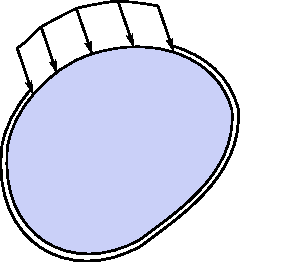
\includegraphics{./images/bcs.pdf}
	\caption{Example figure}
	\label{fig:example}
\end{figure}

\subsection{Preamble, self-defined commands, and acronyms and symbols}

The next chunk of commands in the \texttt{main.tex} file, there is a list of input commands:
\begin{lstlisting}

\usepackage{ifthen}
\usepackage[%
% style=numeric-comp,%
style=nature,%
date=year,%
backend=biber,%
url=false,%
doi=false,%
isbn=false,%
natbib=true,%
sorting=none,%
maxbibnames=99,%
giveninits=true,%
terseinits=true,%
% maxcitenames=1%
]{biblatex}

\usepackage[final]{microtype}
\usepackage{mdframed}

% For displaying LaTeX source code in
% the documentation
\usepackage[final]{listings}
\lstset{
	language=[LaTeX]TeX,
	breaklines=true,
	%basicstyle=\texttt\scriptsize,
	keywordstyle=\color{olive},
	identifierstyle=\color{orange},
}

\usepackage[rightcaption]{sidecap}
\usepackage{rotating}


\usepackage[symbols, acronym, toc, nopostdot, nonumberlist]{glossaries}
\makeglossaries

\relpenalty=10000
\binoppenalty=10000


\endinput

%%%%%%%%%%%%%%%%%%%%%%%%%%%%
% Define your macros here
%%%%%%%%%%%%%%%%%%%%%%%%%%%%

% The command \xspace after defining a word macro adds an extra
% space after the word if needed.
\newcommand{\avhandling}{\textsf{avhandling}\xspace}
\newcommand{\memoir}{\textsf{memoir}\xspace}

\newcommand{\authorname}{Hilde Aas Nøst\xspace}
\newcommand{\authormail}{hilde.nost@gmail.com\xspace}




\endinput

%%%%%%%%%%%%%%%%%%%%%%%%%%%%%%%
% Define your acronyms here
%%%%%%%%%%%%%%%%%%%%%%%%%%%%%%

\newacronym{ntnu}{NTNU}{Norwegian University of Science and Technology}






\endinput

\input{preamble/symbols}
\end{lstlisting}
To tidy things up a bit, loading packages and setting settings are put into a file of their own: \texttt{preamble.tex} which I put into the \texttt{preamble} folder. The names should be self-explicatory.

\paragraph{The preamble.}
Let us take a peak into the preamble settings. The first setting is regarding the references.
By default, the bibliography backend \textsf{biber} is used together with the \textsf{biblatex} package to handle references, as that is currently the most tweakable option.
Other default settings are put in the class file, and they are:
\begin{lstlisting}
\RequirePackage[
  style=nature,	% numbered references
  natbib=true,	% ability to use natbib package macros
  backend=biber,	% defined in class settings
  date=year,
  url=false,	% get rid of urls
  doi=false,	% get rid of dois
  isbn=false,	% get rid of isbns
  sorting=none,	% references chronologically numbered
  maxbibnames=99,
  giveninits=true,	% all first names as initials
  terseinits=true	% no dots after initials
]{biblatex}
\end{lstlisting}
With the exception of the \textbf{style}, \textbf{natbib}, and \textbf{backend} options which need to be set with the class, the rest can be adjusted in the preamble:
\begin{lstlisting}
\ExecuteBibliographyOptions{key=value}
\end{lstlisting}
Check the documentation of the \textsf{biblatex} package for more preamble options.
The documentation also has examples of the various standard styles, but the internet can provide you with several additional styles.
The brave can also create their own.

The \textbf{natbib} option allows us to use the \textsf{natbib} package commands, which is handy. That is the \lstinline{\citep} option for \emph{parenthesis} enclosed citations, such as \citep{Simon1986}.
Another commonly used is the \lstinline{\citet} macro for citations in \emph{text}, such as \citet{Simon1986} wrote something super valuable.

\section{Section without content}

\section{Just adding these to fill out the chapter toc}

\section{Because it looks so tiny otherwise}

\chapter{Class usage}

\intro{How to tweak the look of this very chapter introduction/abstract, and how to turn off
the chapter table of contents.
Also, a note on the todo-notes is added.}

\section{Chapter abstract and table of contents}

I created the command \lstinline{\intro} for the special formatting of the chapter abstract. It is defined in \texttt{avhandling.cls}, and can of course be tweaked to your liking.

In addition, I added a so-called \emph{minitoc} at the end of this chapter abstract.
If you'd like to keep the abstract, but get rid of the minitoc, just delete the \lstinline{\chaptertoc} in the \lstinline{\intro} definition in the \texttt{avhandling.cls} file.

The depth of the table of contents is set to 1, that is, just the section headings are included. Changing \textbf{tocdepth} to 2 will include subsections as well.

\section{Todo-notes}

During the writing process, I used todo-notes in the margin to help keep track of comments\todo{Like so}\todofig.
The package I use, and which is included in this class, is the \textbf{fixme} package\todocite.
I redefined the commands to be more descriptive of how I would use the notes.

There are 3 commands: \lstinline{\todo}, \lstinline{\todocite}, and \lstinline{\todofig}.
The \lstinline{\todo} command needs text input in curly braces, like so: \lstinline|\todo\{Remember this!}|\todocite[Perhaps cite the package manual?].
The other two add by default the text of "citation needed" and "figure wanted".
If you want to describe the problem more, just write of your heart's content in square brackets like so: \lstinline{\todocite[A very very important paper by a very very important author should deffo be cited here.]}. 

\chapter{Tips and tricks}
\label{ch:tips}

\chapter{Conclusion}
\label{ch:conclusion}

Good luck with your thesis writing!

If you have any questions regarding the use of the \textsf{avhandling} class, please contact the author \authorname at \authormail.



%%%%%%%%%%%%%%%%%%%%%%%%%%%%%%%%%
% BACK MATTER
%%%%%%%%%%%%%%%%%%%%%%%%%%%%%%%%%
% Typically contains
% - Bibliography/References
% - Appendices
% - List of acronyms/symbols/etc
%%%%%%%%%%%%%%%%%%%%%%%%%%%%%%%%%

\backmatter
 
% Bibliography/references
% Library file is specified in preamble.tex
\cleardoublepage
\phantomsection
\emergencystretch=1em % Trick for eliminating overfull hboxes in references
\printbibliography[title=References]

% \printglossary[type=symbols,style=long]
\printglossary[type=\acronymtype,style=long]

\end{document}
